\documentclass{article}
%% Chapter 1 Section 10: Exponentiation

\usepackage{amsmath}
\usepackage{palatino}
\usepackage{tikz}

\newcommand{\curry}[1]{\emph{curry}(#1)}
\newcommand{\eval}{\emph{eval}}
\newcommand{\id}{\emph{id}}
\newcommand{\cset}{\mathbf{Set}}
\newcommand{\cseta}{\mathbf{Set}^{\rightarrow}}
\newcommand{\csetset}{\cset \times \cset}
\begin{document}

\begin{enumerate}
\item [1.10.5.1]
\item [1.10.5.2]
  Exponentation in $\csetset$ is componentwise.
  That is, every pair of $\csetset$ objects determines an exponential.
  
  Let $A \times B$ and $C \times D$ be two objects in $\csetset$.
  The exponential of this pair is an object $C^A \times D^B$.
  The function $\eval$  has domain $(C^A \times D^B) \times (A \times B)$ and codomain $C \times D$.
  Application is componentwise.
  The result of $\eval((f, g), (a,b))$ is the pair $(f a, g b)$.

  Then for every arrow $g : E \times (A \times B) \rightarrow C \times D$, we have a unique arrow $\curry{g}$ that maps the $\csetset$ object $E$ to the exponential $C^A \times D^B$.
  This arrow is uniquely determined comoponentwise; because $E$ is itself a pair of $\cset$ objects, each with an exponential, we obtain the $csetset$ object by taking the exponential of the first and second member of the pair.
  
  The entire construction is summarized in the below diagram.
  Parenthesis are inserted for readability.
  \begin{center}
    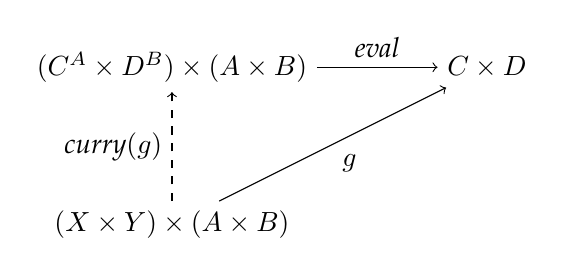
\begin{tikzpicture}
      \node (1) {$(C^A \times D^B) \times (A \times B)$};
      \node[below of=1, yshift=-1cm] (2) {$(X \times Y) \times (A \times B)$};
      \node[right of=1,xshift=3cm] (3) {$C \times D$};
      
      \draw[->] (1) -- node[above] {$\eval$} (3);
      \draw[->] (2) -- node[below right] {$g$} (3);
      \draw[->,dashed] (2) -- node[left] {$\curry{g}$} (1);
    \end{tikzpicture}
  \end{center}

\newpage
\item [1.10.5.3]
  An exponential object in $\cseta$ is a collection of arrows between two $\cseta$ objects.

  An object in $\cseta$ is an arrow $f: A \rightarrow B$ between two sets.
  An arrow between objects $f : A \rightarrow B$ and $f' : A' \rightarrow B'$ in $\cseta$ is a pair of arrows $(a,b)$ where $a : A \rightarrow A'$ and $b: B \rightarrow B'$ are such that $f' \circ a = b \circ f$.
  \begin{center}
    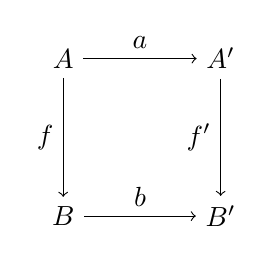
\begin{tikzpicture}
      \node (1) {$A$};
      \node[right of=1,xshift=1cm] (2) {$A'$};
      \node[below of=1,yshift=-1cm] (3) {$B$};
      \node[right of=3,xshift=1cm] (4) {$B'$};
      
      \draw[->] (1) -- node[above] {$a$} (2);
      \draw[->] (1) -- node[left] {$f$} (3);
      \draw[->] (2) -- node[left] {$f'$} (4);
      \draw[->] (3) -- node[above] {$b$} (4);
    \end{tikzpicture}
  \end{center}

  Hence an exponential object $f'^f$ is the collection of all such $\cseta$ arrows $(a,b)$.
  Filling in the canonical diagram for exponentials, we have the following, where $f'' : A'' \rightarrow B''$ is any other object in $\cseta$.
  \begin{center}
    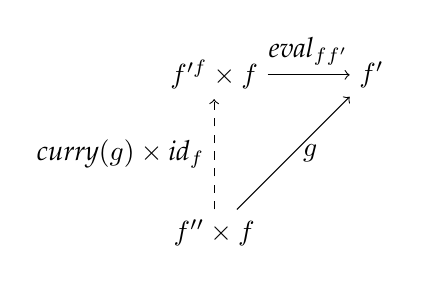
\begin{tikzpicture}
      \node (1) {$f'^f \times f$};
      \node [below of=1,yshift=-1cm] (2) {$f'' \times f$};
      \node [right of=1,xshift=1cm] (3) {$f'$};
      
      \draw[->] (2) -- node [right] {$g$} (3);
      \draw[->,dashed] (2) -- node [left] {$\curry{g} \times \id_f$} (1);
      \draw[->] (1) -- node [above] {$\eval_{ff'}$} (3);
    \end{tikzpicture}
  \end{center}
  Here $\curry{g}$ is the uniquely determined function that brings a $\cseta$ object $f''$ to one of the arrows $f \rightarrow f'$ in the exponential $f'^f$.

\newpage
\item [1.10.5.4]
  To show that $\curry{\eval_{AB}} = \id_{(B^A)}$, we first consider what we know about $\eval_{AB} : B^A \rightarrow B$.
  \begin{center}
    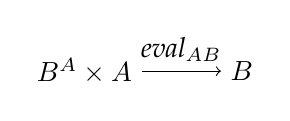
\begin{tikzpicture}
      \node (1) {$B^A \times A$};
      \node [right of=1,xshift=1cm] (3) {$B$};
      
      \draw[->] (1) -- node [above] {$\eval_{AB}$} (3);
    \end{tikzpicture}
  \end{center}
  
  Assuming $B^A$ is an exponential object and that $\eval_{AB}$ is the arrow associated with this exponential, we know that for any other object $C$ and arrow $g : C \times A \rightarrow B$ we have a unique mediating arrow $\curry{g} : C \rightarrow B^A$ such that the following diagram commutes.
  \begin{center}
    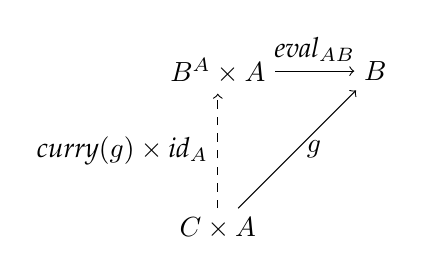
\begin{tikzpicture}
      \node (1) {$B^A \times A$};
      \node [below of=1,yshift=-1cm] (2) {$C \times A$};
      \node [right of=1,xshift=1cm] (3) {$B$};
      
      \draw[->] (2) -- node [right] {$g$} (3);
      \draw[->,dashed] (2) -- node [left] {$\curry{g} \times \id_A$} (1);
      \draw[->] (1) -- node [above] {$\eval_{AB}$} (3);
    \end{tikzpicture}
  \end{center}

  One such possible $g$ is $\eval_{AB}$.
  It takes an object $C = B^A$ to $B$.
  Therefore, there must be a unique arrow $\curry{\eval_{AB}} : B^A \rightarrow B^A$ that makes the diagram commute.
  \begin{center}
    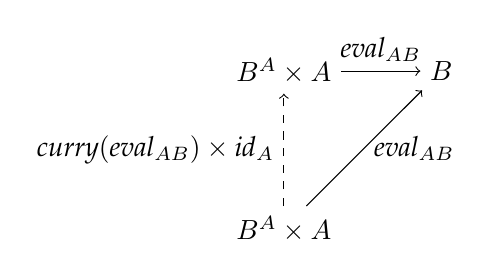
\begin{tikzpicture}
      \node (1) {$B^A \times A$};
      \node [below of=1,yshift=-1cm] (2) {$B^A \times A$};
      \node [right of=1,xshift=1cm] (3) {$B$};
      
      \draw[->] (2) -- node [right] {$\eval_{AB}$} (3);
      \draw[->,dashed] (2) -- node [left] {$\curry{\eval_{AB}} \times \id_A$} (1);
      \draw[->] (1) -- node [above] {$\eval_{AB}$} (3);
    \end{tikzpicture}
  \end{center}
  
  However, $\id_{B^A}$ is another unique arrow that also makes this diagram commute.
  This is more clearly shown if we collapse identical nodes in the diagram.
  \begin{center}
    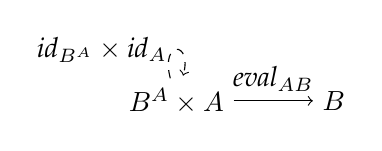
\begin{tikzpicture}
      \node (1) {$B^A \times A$};
      \node [right of=1,xshift=1cm] (3) {$B$};
      
      \draw[->,dashed] (1) edge [loop above] node [left] {$\id_{B^A} \times \id_A$} (1);
      \draw[->] (1) -- node [above] {$\eval_{AB}$} (3);
    \end{tikzpicture}
  \end{center}

  Therefore $\curry{\eval_{AB}} = \id_{B^A}$.

\newpage
\item [1.10.5.5]
  The goal is to show that $(B^A)^{A'}$ is isomorphic to $B^{A \times A'}$ in any cartesian-closed category.

  %% TODO fix the A, A' mixup
  Here goes.\footnote{This feels like a long and indirect argument. I will try again later.}
  Because cartesian-closed categories have exponentials and binary products, we know that for any two objects $A$ and $A'$ both the exponential $A^{A'}$ and product $A \times A'$ exist.
  Construct a function $\eval_1 : A^{A'} \times A' \rightarrow A \times A'$ as $eval_1(f,a) = (f a, a)$.

  This function uniquely determines an arrow $C \rightarrow A^{A'}$ for every function $g : C \times A \rightarrow A \times A'$.
  Let $C$ be $A \times A'$.
  We can easily construct a function $g : (A \times A') \times A \rightarrow A \times A'$ that ignores its second argument and returns its first; therefore, we can use $\eval_1$ to uniquely determine a function $\curry{g} : A \times A' \rightarrow A^{A'}$.
  \begin{center}
    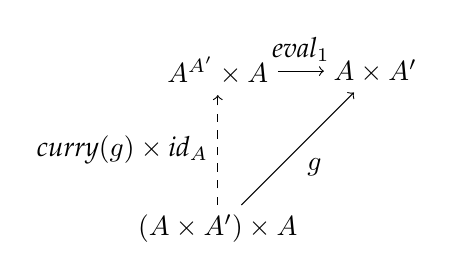
\begin{tikzpicture}
      \node (1) {$A^{A'} \times A$};
      \node [right of=1,xshift=1cm] (2) {$A \times A'$};
      \node [below of=1,yshift=-1cm] (3) {$(A \times A') \times A$};

      \draw[->] (1) -- node[above] {$\eval_1$} (2);
      \draw[->] (3) -- node[below right] {$g$} (2);
      \draw[->,dashed] (3) -- node[left] {$\curry{g} \times \id_A$} (1);
    \end{tikzpicture}
  \end{center}

  With this unique $\curry{g}$, we can construct a unique map $(B^A)^{A'} \rightarrow B^{A \times A'}$ for each arrow $f \in (B^A)^{A'}$.
  Simply compose $f \circ \curry{g}$.
  Call this composition $k$.
  It is one-half of our isomorphism.

  Now $k$ uniquely defines a function $\eval_2 : (B^A)^{A'} \times (A \times A') \rightarrow B$.
  From here, we use the universality of $\eval_2$ to pick out a function $\curry{g'} : B^{A \times A'} \rightarrow (B^A)^{A'}$ in the same manner we chose $\curry{g}$, above.
  Let $g': B^{A \times A'} \times (A \times A') \rightarrow B$ be defined simply as $\eval_3(f,a) = f a$.
  \begin{center}
    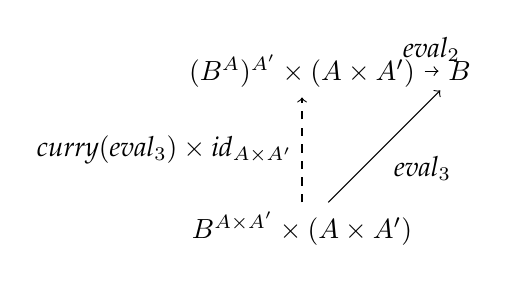
\begin{tikzpicture}
      \node (1) {$(B^A)^{A'} \times (A \times A')$};
      \node [right of=1,xshift=1cm] (2) {$B$};
      \node [below of=1,yshift=-1cm] (3) {$B^{A \times A'} \times (A \times A')$};

      \draw[->] (1) -- node[above] {$\eval_2$} (2);
      \draw[->] (3) -- node[below right] {$\eval_3$} (2);
      \draw[->,dashed] (3) -- node[left] {$\curry{\eval_3} \times \id_{A \times A'}$} (1);
    \end{tikzpicture}
  \end{center}

  This uniquely determines $\curry{\eval_3}$, the inverse of $k$, thus completing the desired isomorphism.

  
\item [1.10.5.6]
\item [1.10.5.7]
\item [1.10.5.8]
\end{enumerate}

\end{document}
